\documentclass[Bachelorarbeit.tex]{subfiles}
\begin{document}
\chapter{Diagramme und Bilder}
\label{chap:diagramme_und_bilder}




\section{Übersicht}
\begin{itemize} 
\item \nameref{sec:mock_ups}
\begin{itemize}
\item \nameref{fig:mockup_android_dashboard}
\item \nameref{fig:wp-startbildschirm}
\item \nameref{fig:Auswahl_Android_Mockups}
\item \nameref{fig:Auswahl_WP_Mockups}
\end{itemize}
\item \nameref{sec:uml_diagramme}
\begin{itemize}
\item \nameref{fig:service_lifecycle}
\end{itemize}

\end{itemize}

\newpage
\chapter*{Mock-Ups}
\label{sec:mock_ups}

\begin{figure}
\centering
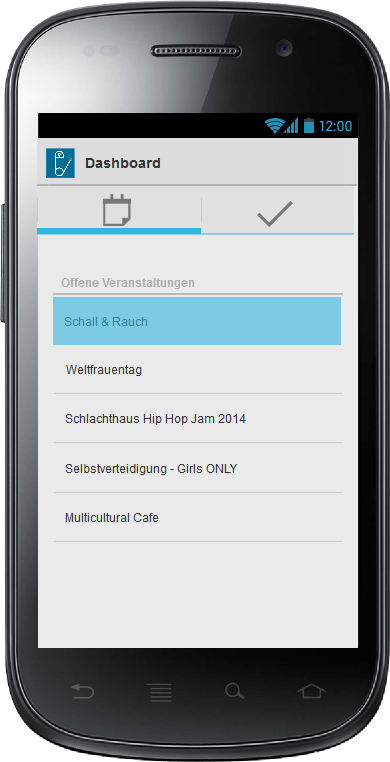
\includegraphics[height=0.7\textheight, angle=90]{./img/mockup_android_dashboard}
\caption[Startbildschirm - Android (Mock-Ups)]{Einsatz von Fragments im Startbildschirm (Mock-Ups)}
\label{fig:mockup_android_dashboard}
\end{figure}
\newpage

\begin{figure}
\centering
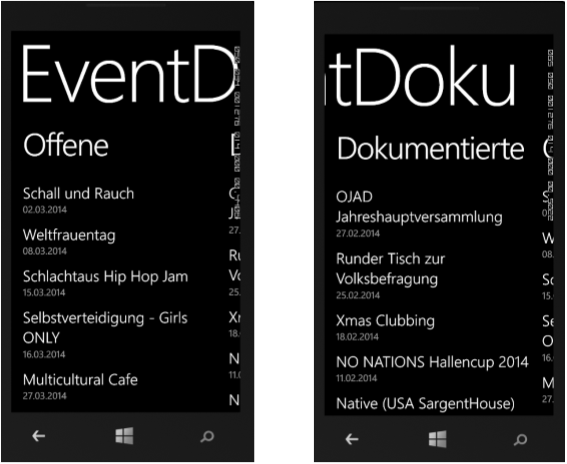
\includegraphics[width=0.8\linewidth]{./img/wp-startbildschirm}
\caption[Startbildschirm - Windows Phone (Mock-Ups)]{Einsatz von Panorama Items im Startbildschirm (Mock-Ups)}
\label{fig:wp-startbildschirm}
\end{figure}


\begin{figure}
\centering
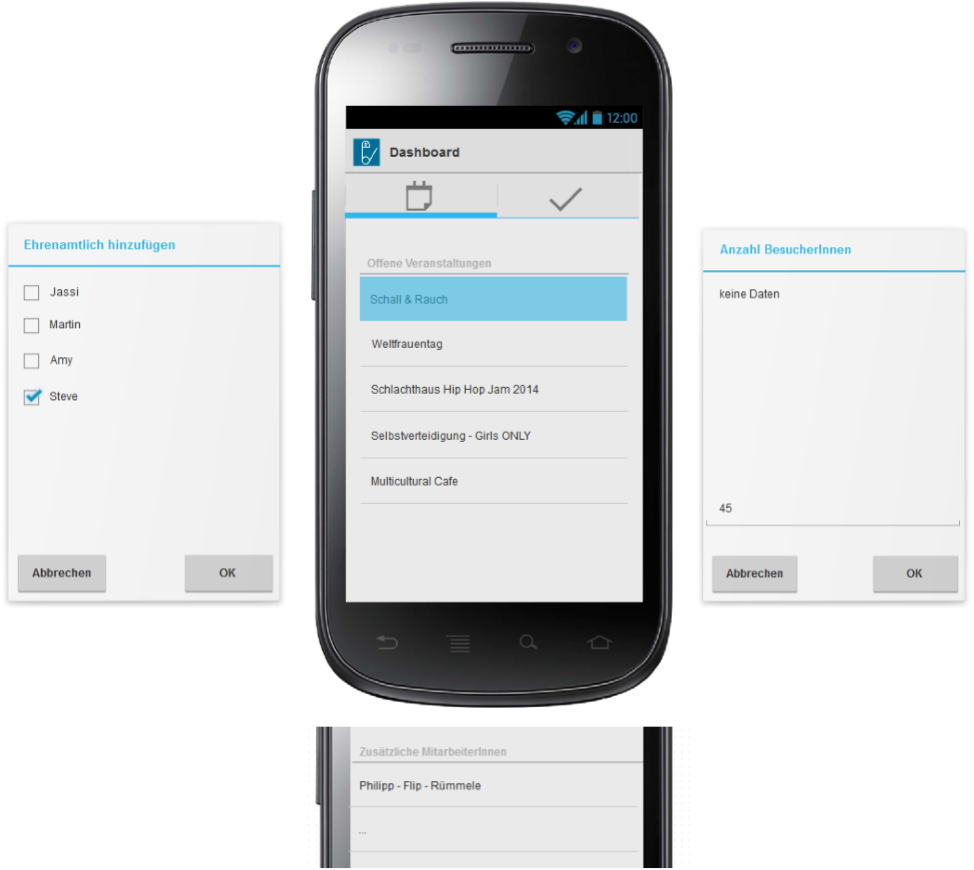
\includegraphics[height=0.7\textheight, angle=90]{./img/Auswahl_Android_Mockups}
\caption{Auswahl der Android-Mock-Ups}
\label{fig:Auswahl_Android_Mockups}
\end{figure}



\begin{figure}
\centering
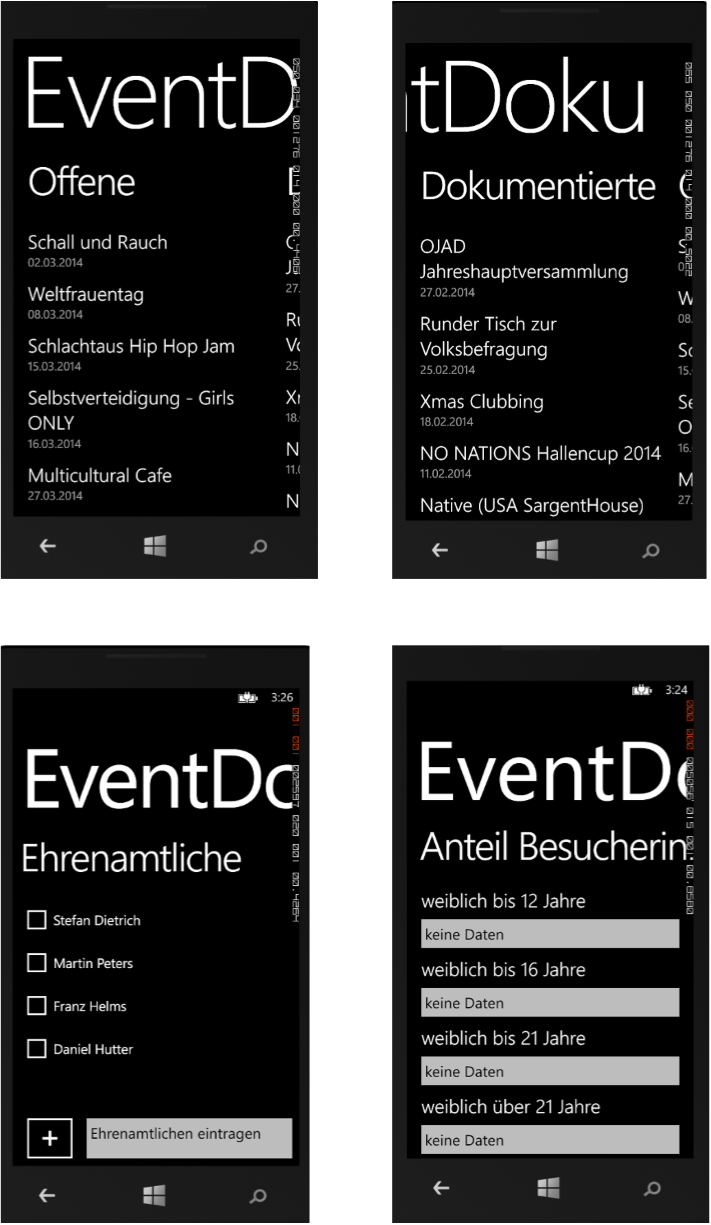
\includegraphics[width=0.9\linewidth]{./img/Auswahl_WP_Mockups}
\caption{Auswahl der Windows Phone-Mock-Ups}
\label{fig:Auswahl_WP_Mockups}
\end{figure}

\newpage

\chapter*{Diagramme}
\label{sec:uml_diagramme}

\begin{figure}
\centering
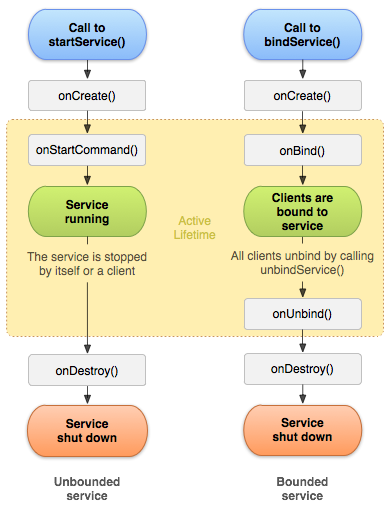
\includegraphics[width=0.7\linewidth]{./img/service_lifecycle}
\caption[Service Lifecycle]{Service Lifecycle - \parencite[Quelle:][]{android_service}}
\label{fig:service_lifecycle}
\end{figure}


\end{document}